%\chapter{Optimizaci\'on de la representaci\'on de datos}

% Approximate nearest neighbors by  deep  hashing on large-scale search: Comparison of representations and retrieval performance 
\chapter{Búsqueda aproximada vía \textit{deep hashing}: Desempeño de métodos de representación y recuperación}

\section{Consideraciones Iniciales}
 
La disponibilidad cada vez mayor de datos en diversos dominios ha creado la necesidad de desarrollar técnicas y métodos para descubrir el conocimiento a partir de volúmenes masivos de datos, motivando muchos trabajos de investigación en bases de datos, \textit{machine learning} y comunidades de recuperación de información. Esto ha impulsado el desarrollo de técnicas escalables y eficientes para organizar y recuperar este tipo de datos. \textit{Similarity search} ha sido el enfoque tradicional para la recuperación de información. Aunque se han propuesto varios algoritmos de búsqueda de similitud para acelerar las consultas de similitud, la mayoría de ellos se ven afectados por la bien conocida \textit{''curse of dimensionality''}. Recuperar datos complejos causa problemas de estabilidad cuando la dimensionalidad de los datos es muy alta \cite{aleman_high_dimensional} .


Se han estudiado diferentes enfoques para resolver el problema de \textit{''curse of dimensionality''}. Una de las líneas de investigación es tratar de evitar el problema de dimensionalidad relajando la precisión de la consulta para acelerar el tiempo de consulta. Potencialmente, este enfoque es factible para aplicaciones que no requieren respuestas exactas y cuya velocidad es más importante que la precisión de búsqueda. Además, la definición del espacio métrico ya conduce a una aproximación de la respuesta verdadera, y por lo tanto una segunda aproximación en el tiempo de búsqueda puede ser aceptable \cite{cit:avez99searching}.

Se propusieron algoritmos de \textit{approximate nearest neighbor search} basados en \textit{hashing} para consultar conjuntos de datos de alta dimensión debido a su alta velocidad de recuperación y bajo costo de almacenamiento. \acf{LSH} \cite{lsh} es una de las recientes técnicas basadas en hash propuestas para organizar y consultar datos de alta dimensión. De hecho, LSH es una de las pocas técnicas que proporciona análisis teóricos sólidos y pérdida predecible de precisión en los resultados. Sin embargo, existe una dependencia en los valores de los parámetros para los esquemas de búsqueda de similitud aproximada basados en LSH, que determinan el número de funciones hash y el número de tablas hash.

Para responder consultas de similitud, \ac{LSH} busca solo regiones, que están representadas por \textit{buckets}, a los que se aplica el hash del objeto de consulta (es decir, los candidatos de los \textit{buckets}  que contienen los objetos del conjunto de datos con una alta probabilidad de similitud con el objeto de consulta). Por lo tanto, no es necesario explorar completamente los datos de índice, y solo los objetos en los candidatos de los \textit{buckets}  que requieren un procesamiento adicional de acuerdo con la condición de consulta (por ejemplo, $ d(x,q) \leq r $) \cite{DBLP:journals/jidm/OcsaS10}.

Hashing produce una representación compacta para documentos, para realizar la tarea como clasificación o base de recuperación en estos códigos hash. Cuando se supervisa el hash, los códigos se entregan usando etiquetas en los datos de entrenamiento. Inspirado por los avances recientes en \acf{CNN} \cite{ImageNet}, muchos métodos mejoran la precisión de la recuperación de similitud al usar CNN como extractor de características y luego crean un código hash compacta de preservación de similitud para una rápida recuperación de imágenes. En un trabajo reciente \cite{kLin:DH}, un método de hashing supervisado entrena el modelo con una capa oculta de \textit{binary-hash} como características para tareas de clasificación de imágenes. Al combinar la extracción de características de imagen y el aprendizaje de \textit{binary-code}, estos métodos han demostrado una precisión de recuperación muy mejorada. Sin embargo, existe un equilibrio entre el error de clasificación y el error de cuantificación: las activaciones de las capas inferiores son más comunes \cite{DBLP:journals/corr/YosinskiCBL14}, por lo que el entrenamiento es más efectivo. Sin embargo, las capas inferiores tienen mapas de activación más grandes (muchos nodos), que son más difíciles de codificar lo que lleva a un compromiso.


\subsection{Approximate Nearest Neighbors \& Deep Hashing}
\subsubsection{Hashing para la Búsqueda del Vecino más Cercano}
En primer lugar, es necesario definir un universo de objetos $ \mathbb{U} $ y una función $ d:\mathbb{U} \times \mathbb{U} \rightarrow \mathbf{R} $ que mida la distancia entre dos objetos de $ \mathbb{U} $. En los espacios métricos, $ S \subseteq \mathbb{U} $ es un conjunto finito de datos que pueden preprocesarse, donde la función $ d() $ mide la disimilitud.

El problema del vecino más cercano, que encuentra el punto más cercano en un conjunto de datos para un punto de consulta específico, es importante en muchas áreas de Ciencia de la Computación. Definimos cuatro problemas de búsqueda de vecinos más cercanos, que usaremos para probar nuestra implementación. Dado un objeto de consulta $ q \in \mathbb{U} $, para recuperar objetos similares a $ q $.

\textbf{Approximate Nearest Neighbor Search $ ANN (q, \varepsilon) $:} encuentra los vecinos más cercanos aproximados de $ q $. La respuesta es aproximadamente correcta con cierta probabilidad, es decir, la probabilidad de éxito $ \delta = 1 - \varepsilon $. Siempre hay una pequeña posibilidad de que otro objeto (la verdadera solución) esté más cerca.

El $ (1+ \varepsilon) -kNNq $ busca los elementos k más similares a $ q $. Supongamos que $ S'= \{s_1', s_2', ..., s_k' \} $ es el conjunto de resultados de la consulta, luego $ \forall s_i'\in S', d (q, s_i') \leq ( 1 + \varepsilon) \times \xi $.

La figura \ref{searchmodelcap5} ilustra el modelo de búsqueda de similitud para la búsqueda ANN utilizando hashing. Cada objeto del conjunto de datos se comprime utilizando códigos hash que generan el nuevo espacio de búsqueda en el espacio reducido. Por lo general, se usa un índice para organizar el conjunto de datos de manera que los objetos cercanos en el espacio original estén juntos bajo cierta probabilidad en el espacio reducido. En el momento de la consulta, el objeto de consulta se asigna a regiones con alta probabilidad de encontrar objetos similares. Finalmente, las regiones de calificación se analizan para informar solo los objetos que satisfacen la condición de consulta.

\begin{figure}[htp]
\label{searchmodelcap5}
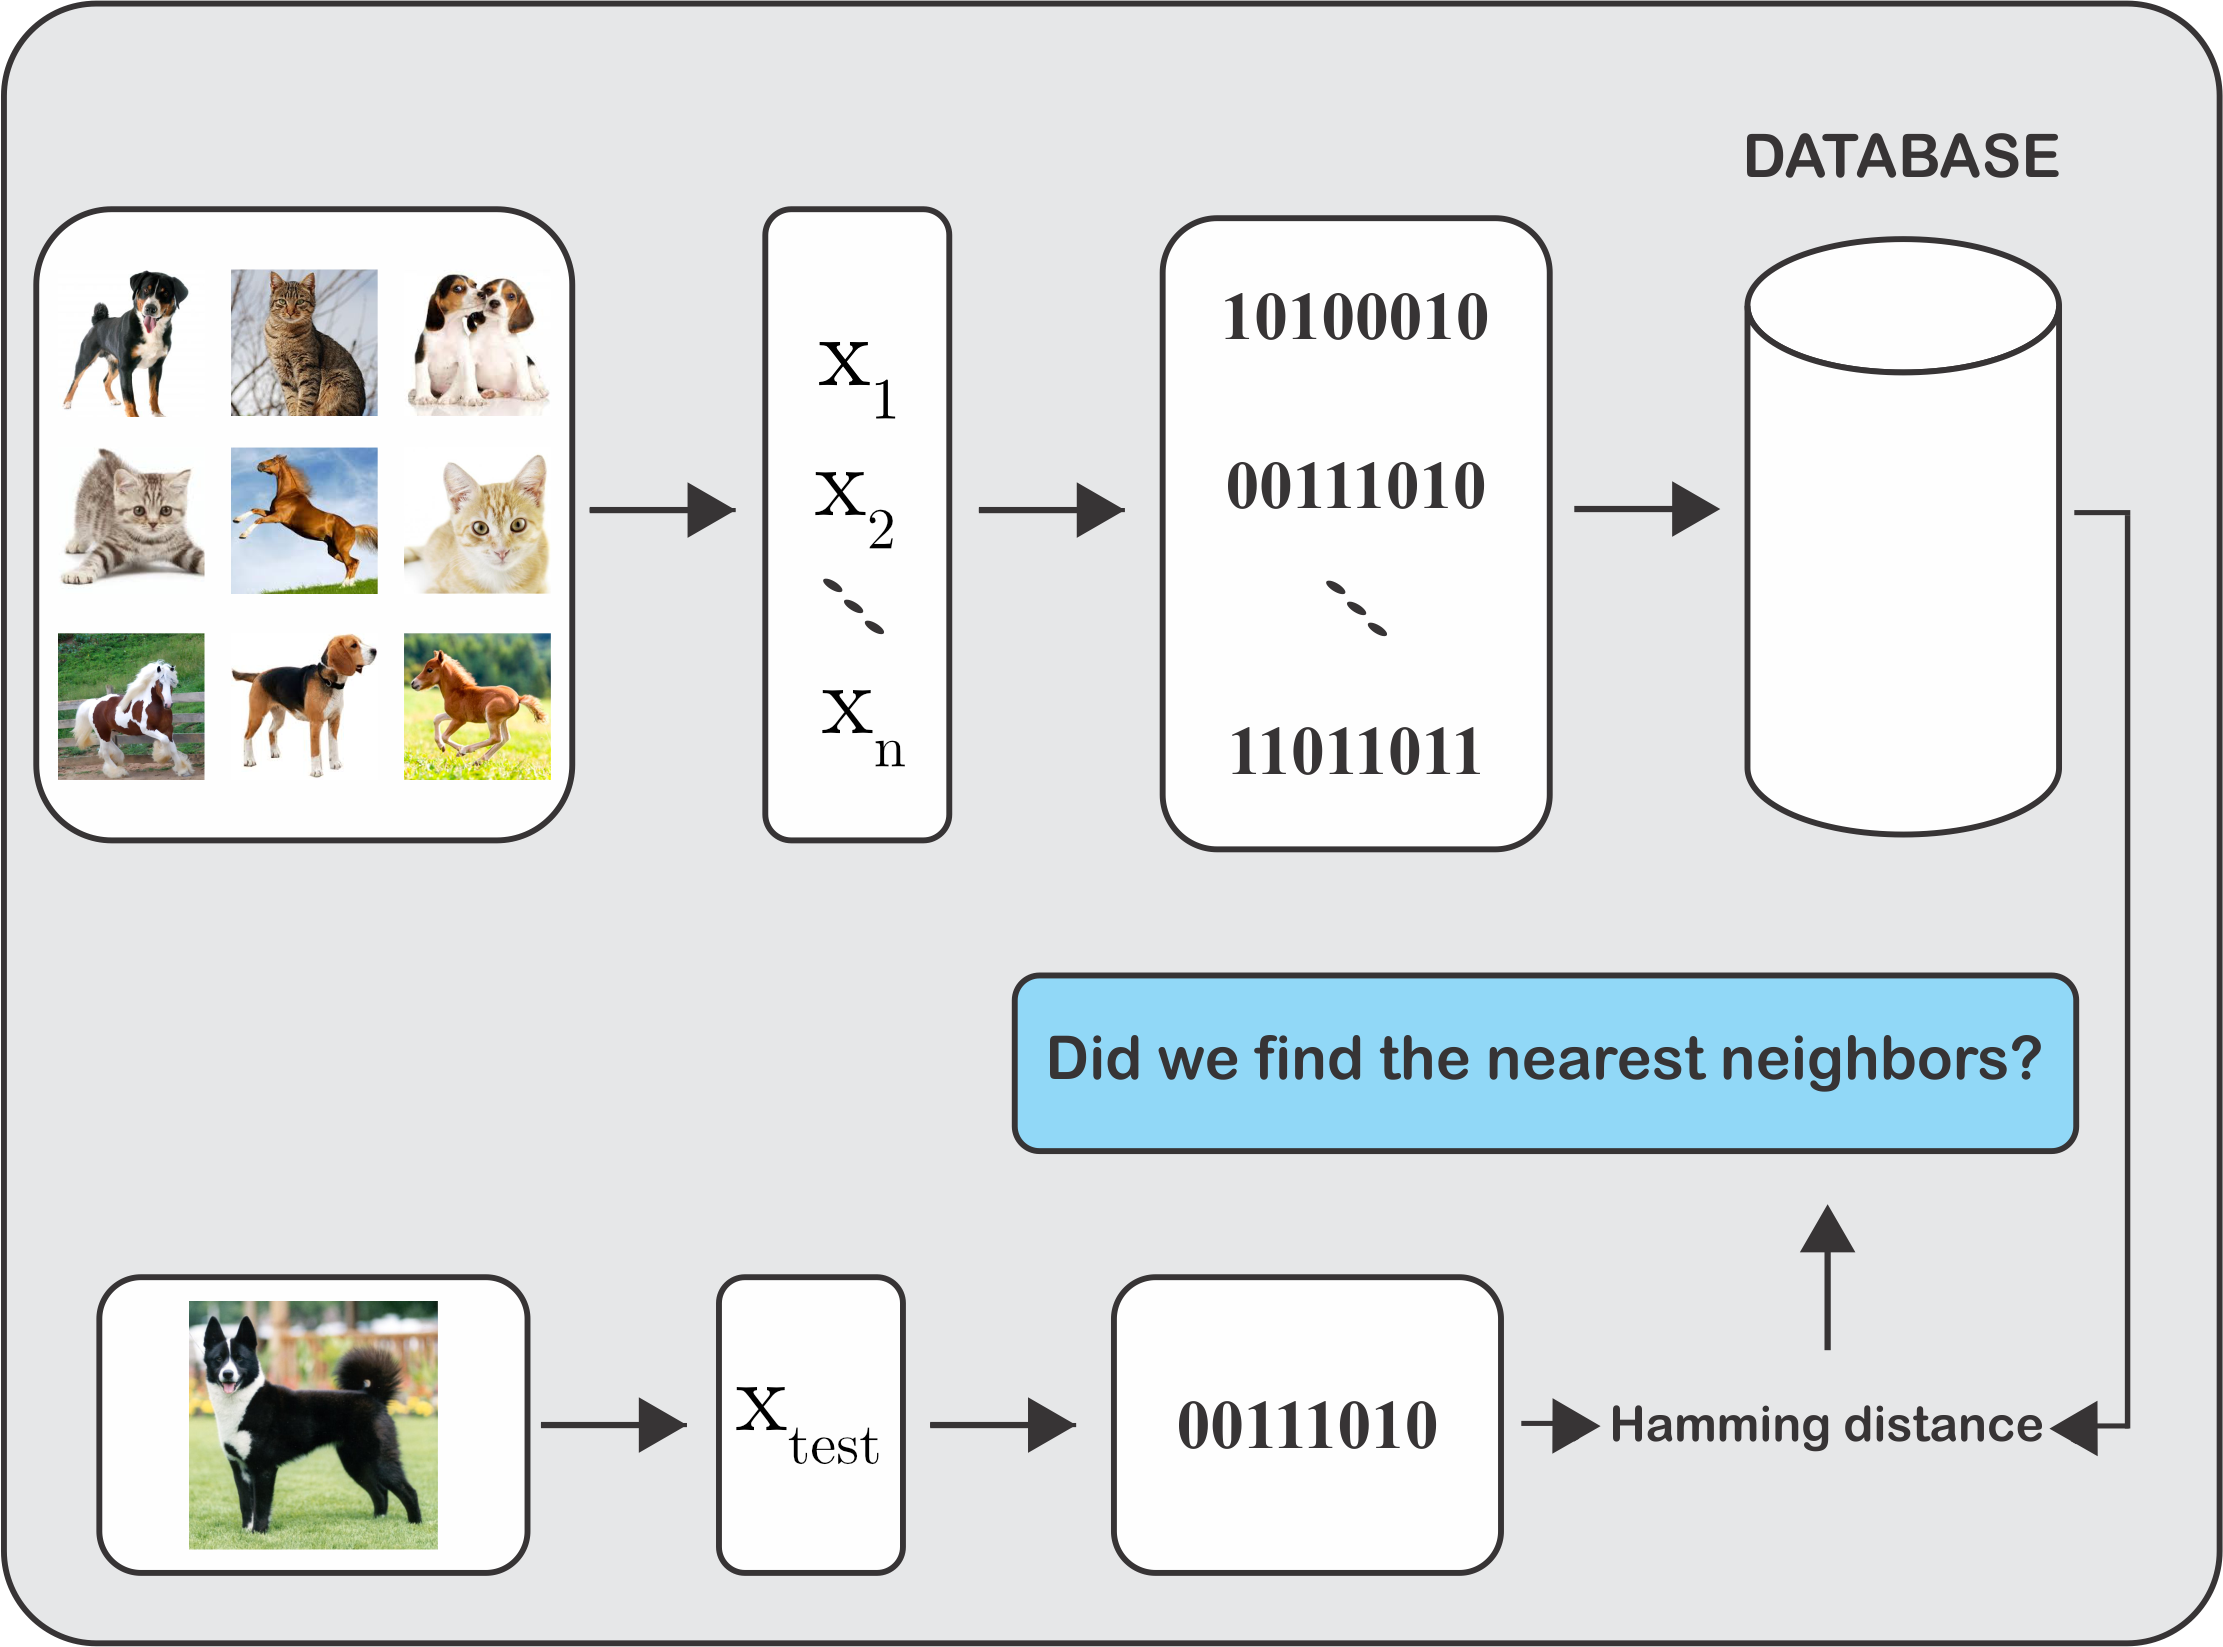
\includegraphics[width=0.7\columnwidth]{chapter5/ima1.png}
\centering
\caption{ Hashing para la búsqueda del vecino más cercano. Comprimir un conjunto de vectores  $(x_i)^{n}_{i=1}, x_i \in \mathbf{R}^d $ }
\end{figure}

\subsubsection{Supervised Hashing}
La figura \ref{supervisedhashingcap5} ilustra un modelo de búsqueda de similitud para Hashing Supervisado. Cada objeto del conjunto de datos se comprime utilizando códigos hash que generan el nuevo espacio de búsqueda en el espacio reducido. Cuando se supervisa el hash, los códigos se entregan usando etiquetas en los datos de entrenamiento.

\begin{figure}[htp]
\label{supervisedhashingcap5}
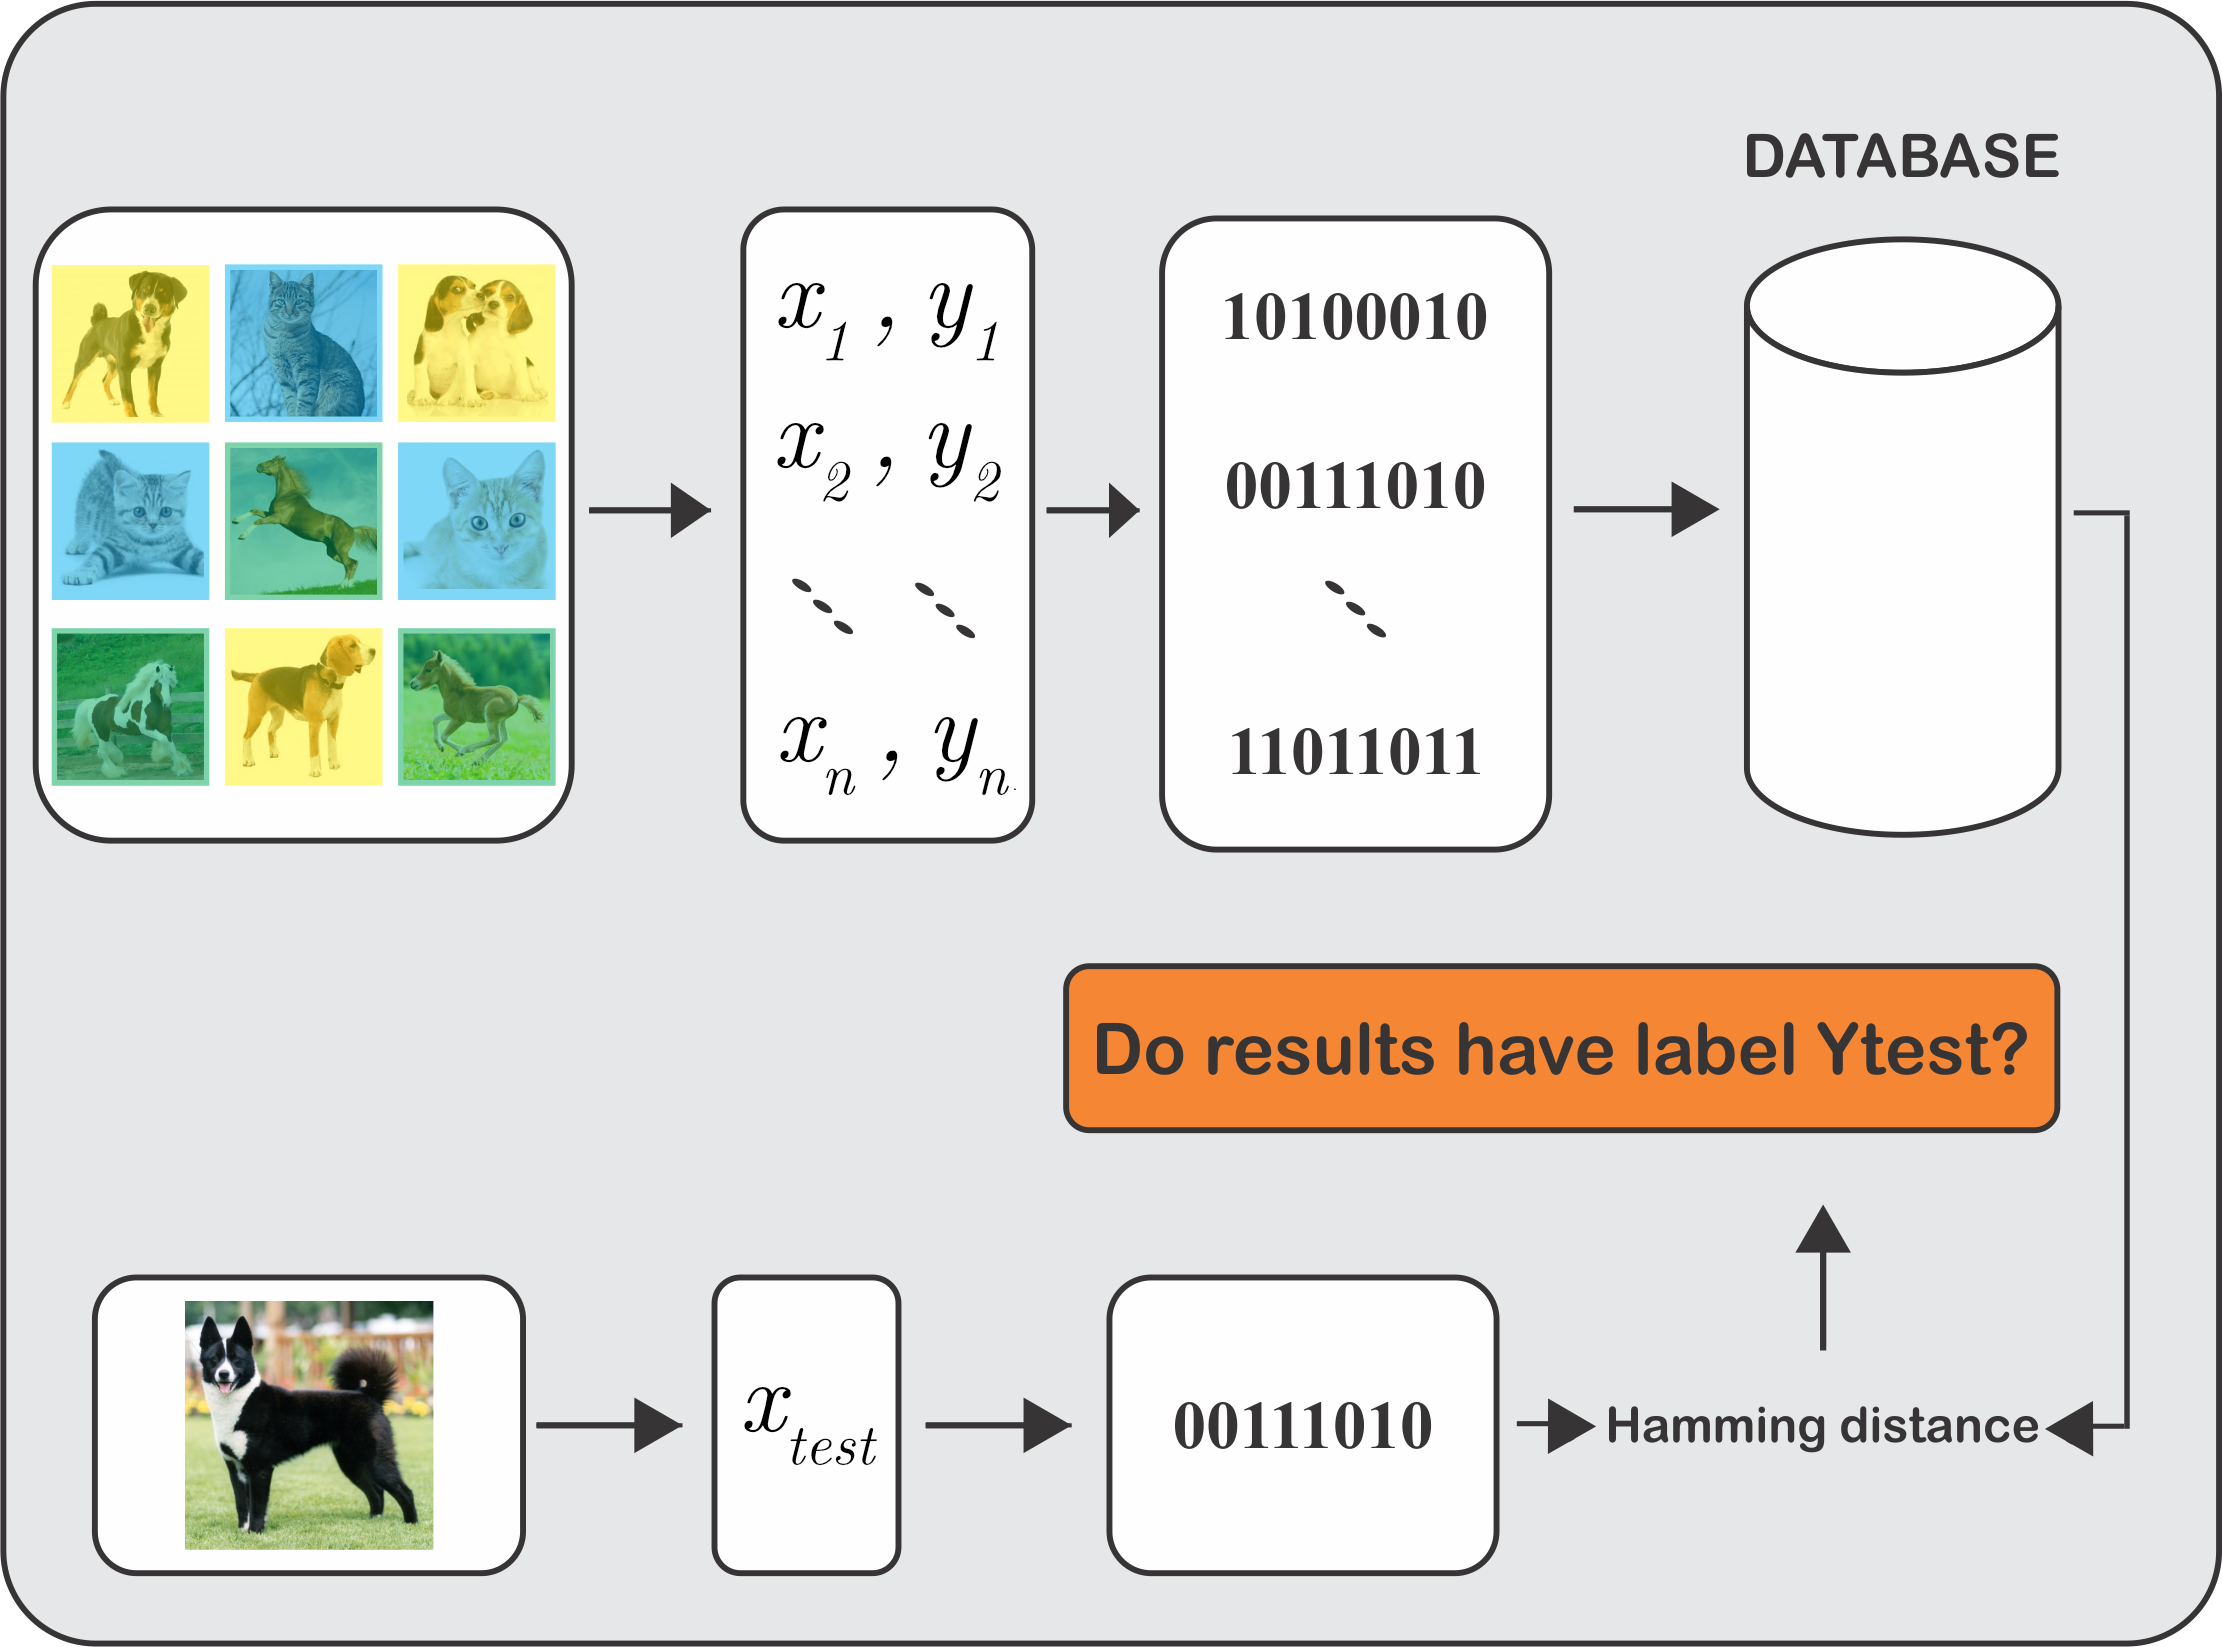
\includegraphics[width=0.7\columnwidth]{chapter5/ima2.png}
\centering
\caption{ Supervised Hashing: comprime un conjunto de vectores y sus etiquetas $((x_i,y_2))^{n}_{i=1}, x_1\in \mathbb{R}^{d}, y_1 \in \{1,...,L\} $.}
\end{figure}

\begin{itemize}
\item Supervised Hashing(SH) $ [1, 2] $: etiquetas $ y_i $ conocido por todos $ x_i (i = 1, ..., n) $ en el conjunto de referencia
\item Semi-supervised hashing (SSH) $ [3, 4] $: etiquetas $ y $ conocido solo por $ n_{label} $ muestras
\end{itemize}

\subsection{Protocolos de evaluación de recuperación}
En esta sección, describimos los protocolos utilizados en la literatura para SSH y SH y explicamos cómo una estrategia simple resuelve eficientemente los problemas similares.

\subsubsection{Protocolos de evaluación de SSH y SH}
SSH consiste en indexar un conjunto de datos de $ n $ imagenes $ \mathcal{I}_{train} $, de los cuales un subconjunto $ \mathcal{I}_{label} \subseteq \mathcal{I}_{train} $ es etiquetado. Pero, SH es el caso extremo $ \mathcal{I}_{label} = \mathcal{I}_{train} $. Si tenemos una imagen de consulta sin etiqueta $ q $, el sistema debe devolver una lista ordenada de imágenes del $ \mathcal{I}_{train} $. Para evaluar, tenemos un conjunto de datos de consultas; el evaluador conoce todas las etiquetas de las consultas, así como las etiquetas en $ \mathcal{I}_{train} $, también en la configuración SSH, y luego una imagen se considera correcta si tiene una misma etiqueta. El rendimiento se mide por precisión o \textit{mean average precision} (mAP).

Entonces, dada una consulta $ q $, si la imagen $ i^{th} $ es correcta para $ q $ definimos $ \delta(q, i) = 1 $, y $ 0 $ de lo contrario. La precisión en el rango $ k $ viene dada por $ P(q, k) = \tfrac{1}{k} {\sum}_{i = 1}^{k} \delta(q, i) $. Denotando por $ cl(q) = {\sum}_{i = 1}^{n} \delta(q, i) $ el número total de imágenes correctas en $ \mathcal{I}_{train} $, y la precisión promedio en $ k $ es $ AP(q, k) = \tfrac{1}{cl(q)} {\sum}_{i = 1}^{k} \delta(q, i) P( q, i) $. El mAP en $ k $ (o simplemente mAP cuando $ k = n $) es el AP promedio sobre todas las consultas de prueba \cite{sablayrolles2016should}.

\subsubsection{Representación de datos y medidas de similitud}\label{sec:methods_reduce}
Se han propuesto muchos métodos en la bibliografía para representar datos complejos con dimensionalidades reducidas, que admiten búsquedas de similitud y tareas de minería de datos. Estos métodos se pueden representar en dos categorías: representaciones de datos adaptables y representaciones de datos no adaptativas \cite{wang13}.

En la representación de \textit{Adaptive Data} tenemos los siguientes métodos: \textit{Singular Value Decomposition} (SVD) que transforma la serie de tiempo $ A_i $ en otra serie de tiempo $ B_i $ de longitud $ n $ cuyos elementos están en orden decreciente \cite{Bettaiah14}. \textit{Principal Component Analysis} (PCA) que involucra procedimientos matemáticos que transforman un número de (posibles) variables de correlación en un número (más pequeño) de variables no correlacionadas, llamadas componentes principales \cite{wekwek}. En PCA, los datos se resumen como una combinación lineal de conjuntos de vectores ortonormales. La PCA actúa de forma similar a los Autoencoders (AE) que aplican la retropropagación estableciendo los valores objetivo para que sean iguales a las entradas $ y(i) = x(i) $ \cite{wekwek}.

Los métodos más comunes utilizados en la representación de datos no adaptativos son: \textit{Discrete Cosine Transformation} (DCT), es una transformación ortonormal real. DCT es similar a \textit{discrete Fourier transform} (DFT) \cite{Faloutsos94}, con la diferencia de que usa funciones de coseno en lugar de senos y cosenos para transformar del dominio de tiempo al dominio de frecuencia \cite{Bettaiah14}. \textit{Discrete Wavelet Transformation} (DWT) procesa datos a diferentes escalas o resoluciones en contraste con DFT \cite{Faloutsos94} donde solo los componentes de frecuencia se consideran  \cite{Bettaiah14}.

Junto con esto, hay más de una docena de medidas de distancia para la búsqueda de similitudes en la literatura. Las medidas de similitud más comunes utilizadas son Euclidean, Manhattan y Minkowski. La distancia euclidiana y la de Manhattan satisfacen algunas propiedades matemáticas: no negatividad, identidad de indiscernibles, simetría, desigualdad de triángulo \cite{han2011data}.

\subsection{Dimensión fractal y reducción de dimensionalidad}
Como se mostró \cite{citeulike:fractal:encoders} que un algoritmo de reducción de dimensionalidad exitoso proyecta los datos en un espacio de características con dimensionalidad cercana a la dimensionalidad fractal (FD) de los datos en el espacio original y conserva las propiedades topológicas.

Por lo tanto, para encontrar la dimensionalidad objetivo ($ m $) necesaria, podemos seguir la siguiente heurística. Podemos comenzar con el valor en $ m_1 = 2^2 $, calcular el FD del nuevo espacio con solo eso, luego incrementar el valor en $ m_2 = 2^3 $, recalcular el FD, y continuar haciendo esto hasta que $ t(m_t = 2^t) $ donde podemos ver un aplanamiento en la dimensión fractal, lo que significa que más características no cambian la dimensionalidad fractal del conjunto de datos.

\subsubsection{Teoría Fractal}
Un fractal se caracteriza por la propiedad de auto-similitud, es decir, es un objeto que presenta aproximadamente las mismas características cuando se analiza en una amplia gama de escalas \cite{DBLP:journals/jidm/TrainaTWF10}. De la Teoría Fractal, \textit{Correlation Fractal Dimension} $ \mathfrak{D} $ es particularmente útil para el análisis de datos, ya que se puede aplicar para estimar la dimensión intrínseca de conjuntos de datos reales que exhiben comportamiento fractal, es decir, conjuntos de datos idénticos o estadísticamente idénticos \cite{DBLP:fractal2016}. Se ha demostrado que, dado un conjunto de $ N $ objetos en un conjunto de datos con una función de distancia $ d(x, y) $, el número promedio de $ k $ vecinos dentro de una distancia dada $ r $ es proporcional a $ r $ elevado a $ \mathfrak{D} $. Por lo tanto, el \textit{pair-count} $ PC(r) $ de pares de elementos dentro de la distancia $ r $ sigue la ley:
\begin{equation}\label{eq:fractal}
       PC(r) = K_p \times r^{\mathfrak{D}}
    \end{equation}
    donde, $ K_p $ es una constante de proporcionalidad, y $ \mathfrak{D} $ es la dimensión fractal de correlación del conjunto de datos.
En consecuencia, un fractal se define por la propiedad de auto-similitud, que es la característica principal que representa exacta o estadísticamente la similitud entre las partes de todo el fractal.

\subsection{Comparación de representaciones de datos}
\subsubsection{Dimensión fractal y reducción de dimensionalidad}\label{sec:fractal-dimension}


% IMAGES ***************
\begin{figure}[htbp]
\centering
\subfigure[Conjunto de datos MNIST]{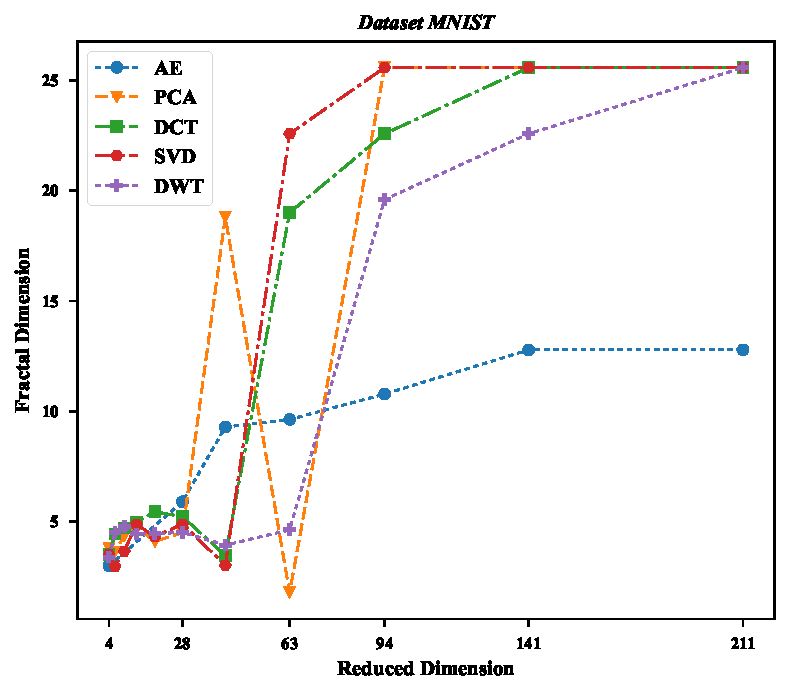
\includegraphics[width=70mm]{chapter5/fig-MNIST.pdf}}
\subfigure[Conjunto de datos CIFAR-10]{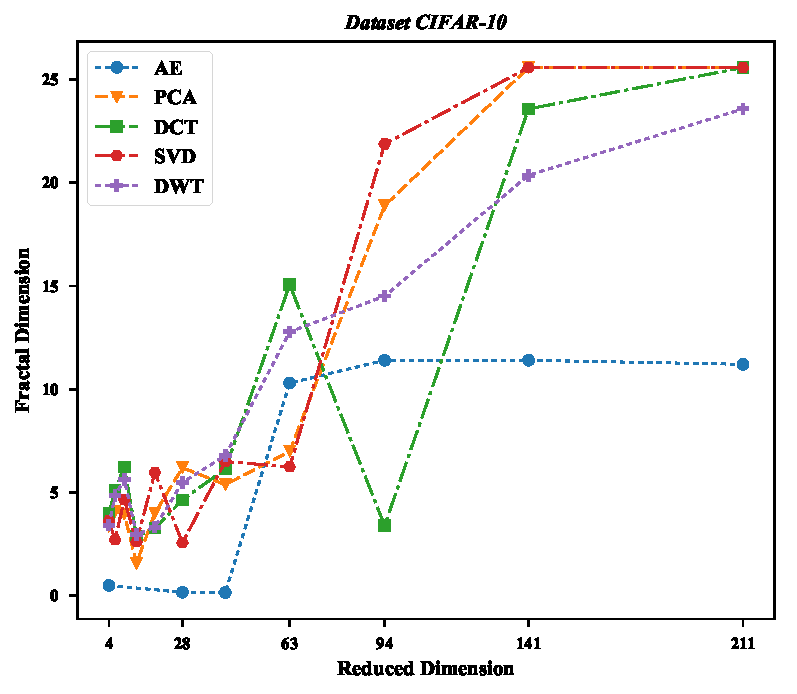
\includegraphics[width=70mm]{chapter5/fig-CIFAR10.pdf}}
\subfigure[Conjunto de datos SVHN]{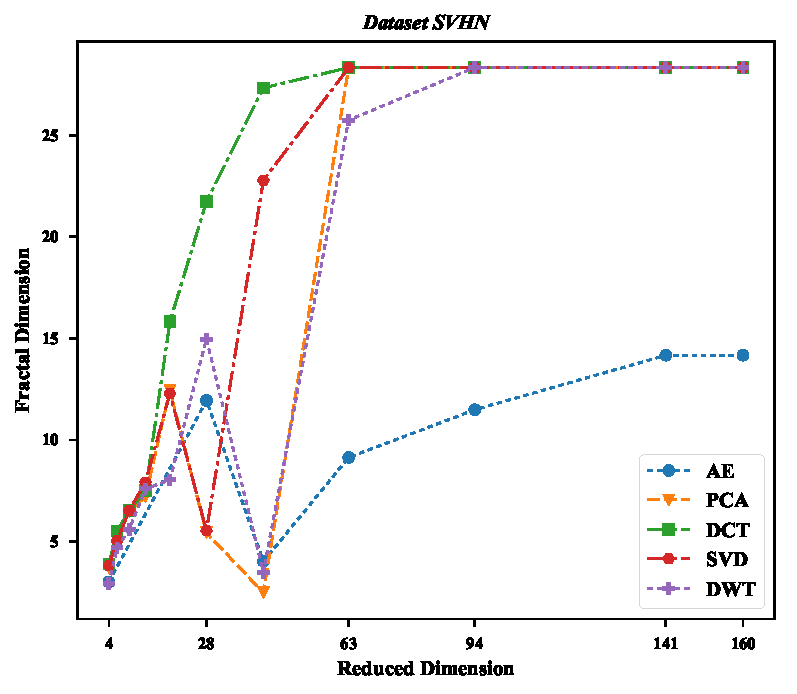
\includegraphics[width=70mm]{chapter5/fig-SVHN.pdf}}
\subfigure[Conjunto de datos AGNEWS]{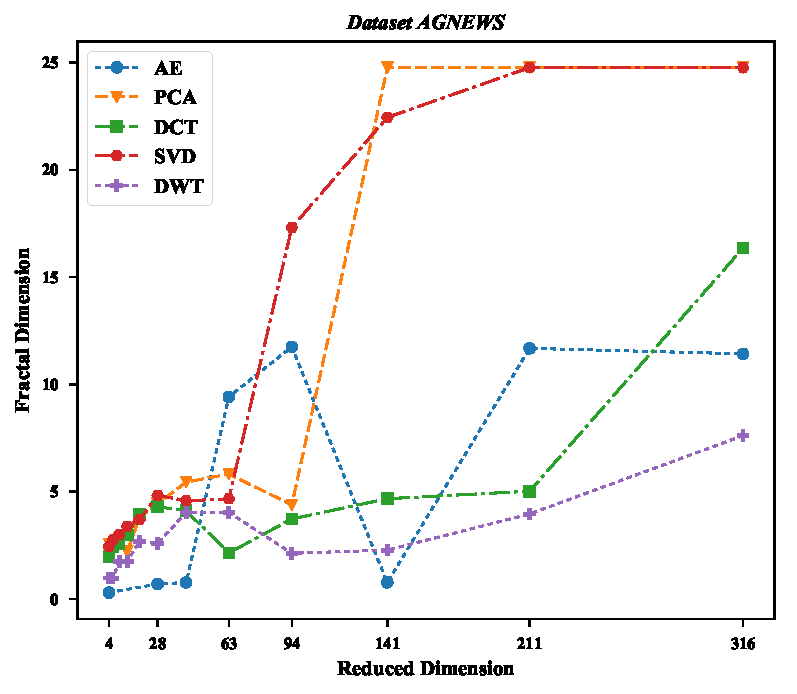
\includegraphics[width=70mm]{chapter5/fig-AGNEWS.pdf}}
\caption{Dimensiones Fractal para diferentes métodos de reducción de dimensionalidad .} \label{fig:datasetscap5}
\end{figure}

Para obtener la representación más general para el aprendizaje, algunos autores sugieren utilizar la salida de la última capa convolucional de la CNN \cite{DBLP:journals/corr/SablayrollesDJU16}. Entonces, en esta investigación, lo usamos como nuestro método de extracción de características. Sin embargo, el espacio reducido donde viven estos datos sigue siendo de gran dimensión. El objetivo de esta sección es encontrar el mejor método de reducción de dimensionalidad y el espacio dimensional más pequeño donde puedan existir los datos sin perder información.

Hemos implementado los métodos de reducción descritos en la sección \ref{sec:methods_reduce}, y los aplicamos en los vectores característicos de los conjuntos de datos MNIST \cite{lecun-mnisthandwrittendigit-2010}, CIFAR-10 \cite{cifar10}, SVHN \cite{svhn} y AgNews \cite{DelCorso:2005:RSN:1060745.1060764}. Para nuestros experimentos, estos vectores de características serán los datos de entrada, y utilizaremos la dimensión fractal para medir el grado de representación de cada nueva dimensión.



Podemos ver la dimensión fractal de cada espacio reducido para cada conjunto de datos en las figuras \ref{fig:datasetscap5}. Con la ayuda de los gráficos, visualizamos que las curvas generadas se estabilizan a medida que aumenta la dimensión reducida, de acuerdo con los experimentos realizados podemos proponer la siguiente hipótesis: "La aproximación de la dimensión reducida óptima es el valor inicial donde la curva del dimensión fractal vs. la dimensión reducida se estabiliza ". Entonces, cualquier reducción de dimensión después del punto de estabilidad, no reducirá la pérdida de información. Para demostrar esto, evaluamos la precisión de clasificación de las dimensiones reducidas, generadas por los métodos PCA y Autoencoders. El método de clasificación que vamos a utilizar será la clasificación KNN. Los resultados se muestran en la tabla \ref{table-result}.


\begin{table}[]
\centering
\caption{Precisión de la clasificación usando KNN-clasificador en conjuntos de datos  MNIST, CIFAR-10, SVHN y Agnews  utilizando  AutoEncoders y PCA como métodos de reducción de dimensionalidad.}
\label{table-result}
\begin{tabular}{c|cc|cccc|}
\cline{2-7}
\multicolumn{1}{l|}{}                           & \multicolumn{2}{c|}{ORIGINAL}                                               & \multicolumn{2}{c|}{AE}                                                       & \multicolumn{2}{c|}{PCA}                                  \\ \cline{2-7} 
\multicolumn{1}{l|}{}                           & \multicolumn{1}{c|}{\cellcolor[HTML]{E6E6E6}Dim.} & Acc.                    & \multicolumn{1}{c|}{\cellcolor[HTML]{E6E6E6}Dim.} & \multicolumn{1}{c|}{Acc.} & \multicolumn{1}{c|}{\cellcolor[HTML]{E6E6E6}Dim.} & Acc.  \\ \hline
\multicolumn{1}{|c|}{}                          & \cellcolor[HTML]{E6E6E6}                          &                         & \cellcolor[HTML]{E6E6E6}63                        & 0.980                     & \cellcolor[HTML]{E6E6E6}42                        & 0.981 \\
\multicolumn{1}{|c|}{}                          & \cellcolor[HTML]{E6E6E6}                          &                         & \cellcolor[HTML]{E6E6E6}141                       & 0.982                     & \cellcolor[HTML]{E6E6E6}94                        & 0.979 \\
\multicolumn{1}{|c|}{\multirow{-3}{*}{MNIST}}   & \multirow{-3}{*}{\cellcolor[HTML]{E6E6E6}800}     & \multirow{-3}{*}{0.982} & \cellcolor[HTML]{E6E6E6}316                       & 0.982                     & \cellcolor[HTML]{E6E6E6}211                       & 0.968 \\ \hline
\multicolumn{1}{|c|}{}                          & \cellcolor[HTML]{E6E6E6}                          &                         & \cellcolor[HTML]{E6E6E6}42                        & 0.902                     & \cellcolor[HTML]{E6E6E6}63                        & 0.897 \\
\multicolumn{1}{|c|}{}                          & \cellcolor[HTML]{E6E6E6}                          &                         & \cellcolor[HTML]{E6E6E6}94                        & 0.894                     & \cellcolor[HTML]{E6E6E6}141                       & 0.889 \\
\multicolumn{1}{|c|}{\multirow{-3}{*}{CIFAR10}} & \multirow{-3}{*}{\cellcolor[HTML]{E6E6E6}4096}    & \multirow{-3}{*}{0.899} & \cellcolor[HTML]{E6E6E6}211                       & 0.898                     & \cellcolor[HTML]{E6E6E6}316                       & 0.868 \\ \hline
\multicolumn{1}{|c|}{}                          & \cellcolor[HTML]{E6E6E6}                          &                         & \cellcolor[HTML]{E6E6E6}63                        & 0.872                     & \cellcolor[HTML]{E6E6E6}28                        & 0.889 \\
\multicolumn{1}{|c|}{}                          & \cellcolor[HTML]{E6E6E6}                          &                         & \cellcolor[HTML]{E6E6E6}141                       & 0.880                     & \cellcolor[HTML]{E6E6E6}63                        & 0.890 \\
\multicolumn{1}{|c|}{\multirow{-3}{*}{SVHN}}    & \multirow{-3}{*}{\cellcolor[HTML]{E6E6E6}1152}    & \multirow{-3}{*}{0.881} & \cellcolor[HTML]{E6E6E6}316                       & 0.879                     & \cellcolor[HTML]{E6E6E6}141                       & 0.880 \\ \hline
\multicolumn{1}{|c|}{}                          & \cellcolor[HTML]{E6E6E6}                          &                         & \cellcolor[HTML]{E6E6E6}94                        & 0.874                     & \cellcolor[HTML]{E6E6E6}63                        & 0.841 \\
\multicolumn{1}{|c|}{}                          & \cellcolor[HTML]{E6E6E6}                          &                         & \cellcolor[HTML]{E6E6E6}211                       & 0.875                     & \cellcolor[HTML]{E6E6E6}141                       & 0.823 \\
\multicolumn{1}{|c|}{\multirow{-3}{*}{AGNEWS}}  & \multirow{-3}{*}{\cellcolor[HTML]{E6E6E6}8704}    & \multirow{-3}{*}{0.867} & \cellcolor[HTML]{E6E6E6}316                       & 0.863                     & \cellcolor[HTML]{E6E6E6}316                       & 0.767 \\ \hline
\end{tabular}
\end{table}

Ahora vamos a hacer un análisis de precisión de clasificación. La idea es trabajar con \textit{nearest neighbor classifier} (1NN) en cada conjunto de datos para evaluar la eficacia de la medida de distancia.

Entonces, comparamos las diferentes varianzas de $ L_p $-norms \cite{sutherland1975introduction}. En la tabla \ref{accuracy-similarities-ae}, podemos ver la precisión para tres dimensiones reducidas mediante Autoencoders de cada conjunto de datos. Encontramos que las distancias \textit{Euclidean} \cite{Gower82} y \textit{Minkowski} tienen un rendimiento similar, y en ambos casos ambas superan en un mínimo a la distancia de \textit{Manhattan}.

\begin{table}[!h]
\centering
\caption{Análisis de precisión de clasificación usando autoencoders para diferentes métricas.}
\label{accuracy-similarities-ae}
\begin{tabular}{|l|l|l|l|l|}
\hline
                                   & \multicolumn{1}{c|}{\textbf{Dim.}} & \multicolumn{1}{c|}{\textbf{L1}} & \multicolumn{1}{c|}{\textbf{L2}} & \multicolumn{1}{c|}{\textbf{L-inf}} \\ \hline
\multirow{3}{*}{\textbf{MNIST}}    & 63                                 & 0,9803                           & \textbf{0,9806}                & \textbf{0,9806}                              \\ \cline{2-5} 
                                   & 141                                & 0,9808                           & \textbf{0,9823}                           & \textbf{0,9823}                              \\ \cline{2-5} 
                                   & 316                                & \textbf{0,9826}                           & 0,9821                           & 0,9821                              \\ \hline
\multirow{3}{*}{\textbf{CIFAR-10}} & 42                                 & 0,9007                           & \textbf{0,9023}                           & \textbf{0,9023}                              \\ \cline{2-5} 
                                   & 94                                 & \textbf{0,8965}                           & 0,8942                           & 0,8942                              \\ \cline{2-5} 
                                   & 211                                & \textbf{0,9009}                           & 0,8982                           & 0,8982                              \\ \hline
\multirow{3}{*}{\textbf{SVHN}}     & 63                                 & 0,8705                           & \textbf{0,8729}                           & \textbf{0,8729}                              \\ \cline{2-5} 
                                   & 141                                & 0,8798                           & \textbf{0,8808}                           & \textbf{0,8808}                              \\ \cline{2-5} 
                                   & 211                                & 0,8781                           & \textbf{0,8795}                           & \textbf{0,8795}                              \\ \hline
\multirow{3}{*}{\textbf{AGNEWS}}   & 94                                 & 0,8714                            & \textbf{0,8748}                        & \textbf{0,8748}                                     \\ \cline{2-5} 
                                   & 211                                & 0,8750                          & \textbf{0,8752}                          & \textbf{0,8752}                                     \\ \cline{2-5} 
                                   & 316                                & \textbf{0,8674}                            & 0,8634                        & 0,8634                                     \\ \hline
\end{tabular}
\end{table}

\subsection{Comparación del rendimiento de recuperación}
En esta sección, describimos las dos tareas de evaluación propuestas en \cite{sablayrolles2016should}, es decir, la recuperación de \textit{unseen classes}. Corresponden a casos de aplicación en 4 grandes conjuntos de datos.

\textbf{Definición del dataset.} en el momento de la prueba, utilizamos clases separadas de un conjunto de datos de clasificación estándar. Al aprender la función de hashing, se supone que se conocen $ 75\% $ de las clases y se usan las clases restantes de $ 25\% $ para evaluar el esquema de codificación/hash. Llamamos a train75/test75 las imágenes de train/test de $ 75\% $ de las clases y train25/test25 las restantes.

\textbf{Protocolo 1: \textit{Retrieval of unseen classes}}, para indexar train25 y usar test25 como consultas, utilizamos el esquema hash. Usamos las etiquetas de train25 solo para evaluación. Esta configuración es como un enfoque de búsqueda de instancias, excepto que las etiquetas de clase dan la verdad. La división train75 - train25 - test25 es el equivalente supervisado de la división de búsqueda - base de datos - consulta en hash no supervisado.
%\textbf{Protocol 1: Retrieval of unseen classes}, to index train25 and use test25 as queries, we use the hashing scheme. We use the labels of train25 for evaluation only. This setup is like an instance search approach except that the class labels give the ground-truth. The train75 - train25 - test25 split is the supervised equivalent of the learn - database - query split in unsupervised hashing. 

El rendimiento se midió en métodos de búsqueda aproximados bien conocidos, E2LSH \cite{multiprobe}, SSDH \cite{kLin:DH}, y también la búsqueda por fuerza bruta. Todos los experimentos se realizaron en un \textit{workstation} con CPU Intel core i7 3.0Ghz (12 núcleos) y 64 Gb de RAM  con cuatro GPU Geforce GTX 1080 con VRAM de 8 Gb cada una.

Realizamos experimentos sobre el modelo propuesto en esta sección (Protocolo 1), utilizando el algoritmo de recuperación de información KNN con k = 100, alimentamos este algoritmo con los espacios reducidos de los conjuntos de datos (MNIST, CIFAR-10, SHVN y AGNews). En la tabla \ref{table:section4_origin_reduction}, podemos ver que el \textit{mean average precision} (mAP) permanece estable a medida que aumenta la dimensión de los datos. Además, el mAP de las dimensiones reducidas está cerca del mAP de los datos de dimensión originales. Por lo tanto, usar una dimensión más grande no mejorará los resultados de la recuperación de información.

\begin{table}[!h]
\centering
\caption{Mean Average Precision(mAP) y el tiempo acumulado para calcular el mAP para diferentes métodos en los conjuntos de datos MNIST, CIFAR-10, SVHN Y AGNEWS. El número k de los vecinos devueltos se establece en 100.}
\label{table:section4_origin_reduction}
\begin{tabular}{l|l|l|l|l|l|l|}
\cline{2-7}
                                                                                 & \multicolumn{3}{l|}{\cellcolor[HTML]{EFEFEF}ORIGINAL}                                                                                              & \multicolumn{3}{l|}{\cellcolor[HTML]{EFEFEF}REDUCCIÓN} \\ \hline
\rowcolor[HTML]{EFEFEF} 
\multicolumn{1}{|l|}{\cellcolor[HTML]{EFEFEF}}                                   & Dim.                                           & mAP                                             & Time                                            & {Dim.}     & {mAp}    & {Time}    \\ \hline
\multicolumn{1}{|l|}{}                                                           &                                                &                                                 &                                                 & 63                & 0.883           & 0.95             \\ \cline{5-7} 
\multicolumn{1}{|l|}{}                                                           &                                                &                                                 &                                                 & 141               & 0.890           & 0.89             \\ \cline{5-7} 
\multicolumn{1}{|l|}{\multirow{-3}{*}{\textbf{MNIST}}}                           & \multirow{-3}{*}{800}                          & \multirow{-3}{*}{0.90}                          & \multirow{-3}{*}{6.53}                          & 316               & 0.88            & 1.56             \\ \hline
\rowcolor[HTML]{EFEFEF} 
\multicolumn{1}{|l|}{\cellcolor[HTML]{EFEFEF}}                                   & \cellcolor[HTML]{EFEFEF}                       & \cellcolor[HTML]{EFEFEF}                        & \cellcolor[HTML]{EFEFEF}                        & 94                & 0.761           & 1.63             \\ \cline{5-7} 
\rowcolor[HTML]{EFEFEF} 
\multicolumn{1}{|l|}{\cellcolor[HTML]{EFEFEF}}                                   & \cellcolor[HTML]{EFEFEF}                       & \cellcolor[HTML]{EFEFEF}                        & \cellcolor[HTML]{EFEFEF}                        & 141               & 0.776           & 2.49            \\ \cline{5-7} 
\rowcolor[HTML]{EFEFEF} 
\multicolumn{1}{|l|}{\multirow{-3}{*}{\cellcolor[HTML]{EFEFEF}\textbf{CIFAR10}}} & \multirow{-3}{*}{\cellcolor[HTML]{EFEFEF}4096} & \multirow{-3}{*}{\cellcolor[HTML]{EFEFEF}0.782} & \multirow{-3}{*}{\cellcolor[HTML]{EFEFEF}13.85} & 211               & 0.776           & 0.98            \\ \hline
\multicolumn{1}{|l|}{}                                                           &                                                &                                                 &                                                 & 63                & 0.780           & 5.23             \\ \cline{5-7} 
\multicolumn{1}{|l|}{}                                                           &                                                &                                                 &                                                 & 141               & 0.790           & 4.56             \\ \cline{5-7} 
\multicolumn{1}{|l|}{\multirow{-3}{*}{\textbf{SVHN}}}                            & \multirow{-3}{*}{1152}                         & \multirow{-3}{*}{0.816}                         & \multirow{-3}{*}{35.61}                         & 211               & 0.780           & 6.19             \\ \hline
\rowcolor[HTML]{EFEFEF} 
\multicolumn{1}{|l|}{\cellcolor[HTML]{EFEFEF}}                                   & \cellcolor[HTML]{EFEFEF}                       & \cellcolor[HTML]{EFEFEF}                        & \cellcolor[HTML]{EFEFEF}                        & 94                & 0.785           & 0.63             \\ \cline{5-7} 
\rowcolor[HTML]{EFEFEF} 
\multicolumn{1}{|l|}{\cellcolor[HTML]{EFEFEF}}                                   & \cellcolor[HTML]{EFEFEF}                       & \cellcolor[HTML]{EFEFEF}                        & \cellcolor[HTML]{EFEFEF}                        & 211               & 0.788           & 0.76             \\ \cline{5-7} 
\rowcolor[HTML]{EFEFEF} 
\multicolumn{1}{|l|}{\multirow{-3}{*}{\cellcolor[HTML]{EFEFEF}\textbf{AGNEWS}}}  & \multirow{-3}{*}{\cellcolor[HTML]{EFEFEF}8704} & \multirow{-3}{*}{\cellcolor[HTML]{EFEFEF}0.775} & \multirow{-3}{*}{\cellcolor[HTML]{EFEFEF}15.95} & 316               & 0.788           & 0.67             \\ \hline
\end{tabular}
\end{table}     

Finalmente, utilizamos Autoencoders con cinco capas, para generar dimensiones reducidas de los conjuntos de datos (MNIST, CIFAR-10, SHVN y AGNews). Las dimensiones (141,141,141 y 211), respectivamente, son las aproximaciones del mejor espacio reducido. Además, comparamos el mejor espacio reducido frente a la dimensión original y una dimensión más pequeña. Nuestro resultado en la Tabla \ref{table:section4_presicion1000} muestra que los espacios mejor reducidos obtienen una precisión cercana a la dimensión original.

\begin{table}[!h]
\centering
\caption{Precisión 1000-NN y tiempo acumulado para diferentes métodos en los conjuntos de datos MNIST, CIFAR-10, SVHN y AGNEWS. El número k de los vecinos devueltos se establece en 1000.}
\label{table:section4_presicion1000}
\begin{tabular}{l|l|l|l|}
\cline{2-4}
                                                                        &               & 1000-NN & Time  \\ \hline
\multicolumn{1}{|l|}{}                                                  & SSDH(D=48)    & 0.514   & 3.802 \\ \cline{2-4} 
\multicolumn{1}{|l|}{}                                                  & E2LSH(D=800)  & 0.873   & 9.531  \\ \cline{2-4} 
\multicolumn{1}{|l|}{\multirow{-3}{*}{MNIST}}                           & E2LSH(D=141)  & 0.688   & 4.152 \\ \hline
\rowcolor[HTML]{EFEFEF} 
\multicolumn{1}{|l|}{\cellcolor[HTML]{EFEFEF}}                          & SSDH(D=128)   & 0.437   & 3.972 \\ \cline{2-4} 
\rowcolor[HTML]{EFEFEF} 
\multicolumn{1}{|l|}{\cellcolor[HTML]{EFEFEF}}                          & E2LSH(D=4096) & 0.759   & 6.85 \\ \cline{2-4} 
\rowcolor[HTML]{EFEFEF} 
\multicolumn{1}{|l|}{\multirow{-3}{*}{\cellcolor[HTML]{EFEFEF}CIFAR10}} & E2LSH(D=141)  & 0.493   & 4.223 \\ \hline
\multicolumn{1}{|l|}{}                                                  & SSDHI(D=63)   & 0.332   & 11.45 \\ \cline{2-4} 
\multicolumn{1}{|l|}{}                                                  & E2LSH(D=1152) & 0.780   & 19.723  \\ \cline{2-4} 
\multicolumn{1}{|l|}{\multirow{-3}{*}{SVHN}}                            & E2LSH(D=141)  & 0.634   & 12.56 \\ \hline
\rowcolor[HTML]{EFEFEF} 
\multicolumn{1}{|l|}{\cellcolor[HTML]{EFEFEF}}                          & SSDH(D=128)   & 0.384   & 3.217 \\ \cline{2-4} 
\rowcolor[HTML]{EFEFEF} 
\multicolumn{1}{|l|}{\cellcolor[HTML]{EFEFEF}}                          & E2LSH(D=8704) & 0.790   & 13.763 \\ \cline{2-4} 
\rowcolor[HTML]{EFEFEF} 
\multicolumn{1}{|l|}{\multirow{-3}{*}{\cellcolor[HTML]{EFEFEF}AGNEWS}}  & E2LSH(D=211)  & 0.590   & 3.321 \\ \hline
\end{tabular}
\end{table}

\section{Conclusions}
Presentamos experimentos exhaustivos que comparan métodos recientes de \textit{deep hashing} que permitieron obtener mejores representaciones del espacio de datos con un menor costo computacional para obtener una mejor precisión al calcular los mejores parámetros de datos. Hemos explorado las correlaciones entre CNN usando la teoría fractal. Para optimizar estos parámetros, utilizamos diferentes métodos de reducción de dimensionalidad que proyectan el conjunto de datos en un espacio de características con dimensionalidad cercana a la dimensionalidad fractal (FD) de los datos en el espacio original. Presentamos una descripción general de estas diferentes técnicas y presentamos nuestro experimento comparativo para representación de datos y rendimiento de recuperación. Los resultados empíricos muestran las capacidades de la teoría Fractal para encontrar el subespacio óptimo del conjunto de datos, podemos encontrar una configuración óptima para el proceso de aprendizaje e indexación. Además, pudimos sintonizar métodos de \textit{deep hashing}, basados en la teoría fractal, que nos permite encontrar los valores de parámetros óptimos. Además, podemos estimar estos parámetros en tiempo lineal debido a que depende del cálculo de la dimensión fractal.